
\documentclass[10pt,a4paper,twocolumn,twoside]{article}
\usepackage[utf8]{inputenc}
\usepackage[catalan]{babel}
\usepackage{multicol}
\usepackage{graphicx}
\usepackage{fancyhdr}
\usepackage{times}
\usepackage{titlesec}
\usepackage{multirow}
\usepackage{lettrine}
\usepackage[top=2cm, bottom=1.5cm, left=2cm, right=2cm]{geometry}
\usepackage[figurename=Fig.,tablename=TAULA]{caption}
\captionsetup[table]{textfont=sc}
% \usepackage{urlbst}
\usepackage{hyperref}


\author{\LARGE\sffamily Pol Colomer Campoy}
\title{\Huge{\sffamily Desenvolupament d'una Plataforma per a l'Anàlisi i Generació de Partitures Musicals a partir d'Àudio Multitrack}}


\newcommand\blfootnote[1]{%
  \begingroup
  \renewcommand\thefootnote{}\footnote{#1}%
  \addtocounter{footnote}{-1}%
  \endgroup
}

%
%\large\bfseries\sffamily
\titleformat{\section}
{\large\sffamily\scshape\bfseries}
{\textbf{\thesection}}{1em}{}

\begin{document}

\fancyhead[LO]{\scriptsize AUTOR: TÍTOL DEL TREBALL}
\fancyhead[RO]{\thepage}
\fancyhead[LE]{\thepage}
\fancyhead[RE]{\scriptsize EE/UAB TFG INFORMÀTICA: TÍTOL (ABREUJAT SI ÉS MOLT LLARG)}

\fancyfoot[CO,CE]{}

\fancypagestyle{primerapagina}
{
   \fancyhf{}
   \fancyhead[L]{\scriptsize TFG EN ENGINYERIA INFORMÀTICA, ESCOLA D'ENGINYERIA (EE), UNIVERSITAT AUTÒNOMA DE BARCELONA (UAB)}
   \fancyfoot[C]{\scriptsize ``Mes'' de 20xx, Escola d'Enginyeria (UAB)}
}

%\lhead{\thepage}
%\chead{}
%\rhead{\tiny EE/UAB TFG INFORMÀTICA: TÍTOL (ABREUJAT SI ÉS MOLT LLARG)}
%\lhead{ EE/UAB \thepage}
%\lfoot{}
%\cfoot{\tiny{Mes 2024, Escola d'Enginyeria (UAB)}}
%\rfoot{}
\renewcommand{\headrulewidth}{0pt}
\renewcommand{\footrulewidth}{0pt}
\pagestyle{fancy}

%\thispagestyle{myheadings}
\twocolumn[\begin{@twocolumnfalse}

%\vspace*{-1cm}{\scriptsize TFG EN ENGINYERIA INFORMÀTICA, ESCOLA D'ENGINYERIA (EE), UNIVERSITAT AUTÒNOMA DE BARCELONA (UAB)}

\maketitle

\thispagestyle{primerapagina}
%\twocolumn[\begin{@twocolumnfalse}
%\maketitle
%\begin{abstract}
\begin{center}
\parbox{0.915\textwidth}
{\sffamily
\textbf{Resum--}
TODO: Aconseguir separar pistes d’àudio donat un àudio multitrack i obtenir les notes de cada pista per posteriorment generar la partitura de la mateixa. Estudiar els resultats obtinguts per diferents algoritmes amb diferents configuracions i combinacions d’àudios.
\\
\\
\textbf{Paraules clau-- } Paraules clau del treball, màxim 2 línies . .... ........ ........... .......... ..  TODO Multitrack, .\\
\\
%\end{abstract}
%\bigskip
%\begin{abstract}
\bigskip
\\
\textbf{Abstract--} 
TODO: To separate audio tracks by giving a multitrack audio and obtain the notes of each track to later generate the score of it. Study the results obtained by different algorithms with different configurations and audio combinations.
\\
\\
\textbf{Keywords-- } Versió en anglès de les paraules clau. .... ........ ........... .......... ..  ... ..... .... ........ ........... .......... ..  ... ..... .... ........ ........... .................. ..\\
}

\bigskip

{\vrule depth 0pt height 0.5pt width 4cm\hspace{7.5pt}%
\raisebox{-3.5pt}{\fontfamily{pzd}\fontencoding{U}\fontseries{m}\fontshape{n}\fontsize{11}{12}\selectfont\char70}%
\hspace{7.5pt}\vrule depth 0pt height 0.5pt width 4cm\relax}

\end{center}

\bigskip
%\end{abstract}
\end{@twocolumnfalse}]

\blfootnote{$\bullet$ E-mail de contacte: Pol.ColomerC@autonoma.cat}
\blfootnote{$\bullet$ Menció realitzada: Computació}
\blfootnote{$\bullet$ Treball tutoritzat per: Felipe Lumbreras (departament - CVC)}
\blfootnote{$\bullet$ Curs 2023/2024}


\section{Introducció - Context del treball}
\label{sec:intro}

\lettrine[lines=3]{E}{n} els darrers anys, el camp de l'enginyeria informàtica ha experimentat un notable avanç en el tractament del senyal d'àudio i en l'anàlisi musical automatitzada. El meu projecte d'enginyeria informàtica, que implica la separació d'instruments, la generació de partitures i la creació de tutorials visuals, s'ubica en la intersecció de diverses àrees de recerca i desenvolupament. La meva principal motivació és adquirir pràctica, comprensió i realitzar una investigació en l'àmbit de l'àudio, ja que durant la meva carrera, és un dels temes que han quedat menys explorats. D'aquesta manera, pretenc enriquir la meva experiència com a estudiant en aquest àmbit.


\section{Objectius}
\label{sec:objectius}

L'objectiu principal d'aquest projecte és aconseguir la separació de pistes d'àudio d'un arxiu multitrack i obtenir les notes musicals de cada pista per a la posterior generació de la seva partitura. A continuació, es detallen els objectius ramificats en forma d'arbre:

\begin{enumerate}
    \item Recopilar i preparar les dades necessàries per al desenvolupament del projecte, incloent-hi Toy problems, problemes complexes i àudios reals.
    
    \item Desenvolupar algoritmes i tècniques per a la separació de pistes d'àudio tant amb tècniques clàssiques com actuals i realitzar un estudi i anàlisi dels resultats.
    \begin{enumerate}
        \item Desenvolupar l'algorisme ICA.
        \item Desenvolupar un model U-Net d'una CNN amb Machine Learning i les diverses formes de processament d'àudio: Spectrum, Cepstrum, MFCC i GFCC.
    \end{enumerate}
    \item Obtindre les notes musicals de cada pista separada per tal de transcriure-la.
    \item Generar la partitura musical de cada pista
\end{enumerate}

\section{Tasques}
\label{sec:tasques}

Per assolir els objectius establerts, s'han definit les següents tasques, les quals estan dissenyades per abordar de manera efectiva els diversos aspectes del projecte:

\begin{enumerate}
    \item Recopilació de dades i preparació: (5 setmanes en total (paral·lel)
    \begin{enumerate}
        \item Investigar i seleccionar una varietat de toy problems representatius dels casos d'ús. (1 setmana)
        \item Recopilar una col·lecció d'arxius MIDI de diverses cançons juntament amb les seves partitures corresponents. (1 setmana)
        \item Obtindre àudios multitrack de concerts amb soroll ambient del públic per a casos més desafiant i variats. (1 setmana)
        \item Pre-processar i netejar les dades recopilades per garantir la seva qualitat i coherència. (2 setmanes)
    \end{enumerate}
    
    \item Desenvolupament d'algoritmes i tècniques per a la separació de pistes d'àudio:
    \begin{enumerate}
        \item Realitzar una revisió exhaustiva per identificar i comprendre els algoritmes clàssics i tècniques de Deep Learning més adequats per a la separació de pistes d'àudio. (2 setmanes)
        \item Implementar una gamma d'algoritmes clàssics com ara Independent Component Analysis (ICA), Principal Component Analysis (PCA), Non-negative Matrix Factorization (NMF) i algorismes de filtratge per explorar la seva eficàcia en la separació de pistes. (3 setmanes)
        \item Investigar i experimentar amb les tècniques de deep learning, incloent-hi Xarxes Neuronals Convolucionals (CNNs), Xarxes Neuronals Recurrents (RNNs), U-Net, Wave-U-Net i Deep Clustering, per millorar la qualitat i la precisió de la separació de pistes. (4 setmanes)
        \item Avaluar i comparar el rendiment dels diferents algoritmes i tècniques implementades utilitzant mètriques rellevants com la relació senyal-soroll (SNR), la separació de font de bescanvi (SiSdr) i la puntuació de seguiment de referència (SAR). (2 setmanes)
    \end{enumerate}
    
    \item Obtenció de les notes musicals de cada pista separada:
    \begin{enumerate}
        \item Investigar i desenvolupar mètodes d'extracció de característiques i anàlisi musical per obtenir les notes musicals de cada pista separada. (1 setmana)
        \item Implementar algoritmes d'anàlisi de freqüències, reconeixement de patrons i sincronització temporal per a l'extracció precisa de les notes musicals. (3 setmanes)
        \item Provar i ajustar els mètodes d'extracció de notes en diferents escenaris i tipus de pistes d'àudio. (1 setmana)
    \end{enumerate}
    
    \item Generació de partitures:
    \begin{enumerate}
        \item Desenvolupar algoritmes i processos per a la generació automàtica de partitures a partir de les notes musicals obtingudes. (3 setmanes)
        \item Implementar funcionalitats addicionals com la detecció de claus i la transcripció automàtica de les partitures generades. (2 setmanes)
        \item Validar les partitures generades mitjançant comparació amb les partitures originals i avaluació manual de la seva qualitat musical. (1 setmana)
    \end{enumerate}
    \item Documentació del projecte:
    \begin{enumerate}
        \item Preparar un Jupyter Notebook exhaustiu que descriu el procés complet del projecte, des de la recopilació de dades fins a la generació de partitures, incloent-hi explicacions detallades, codi font i visualitzacions. (2 setmanes)
        \item Crear una documentació detallada que explica els passos realitzats, els resultats obtinguts, les conclusions del projecte i les possibilitats de desenvolupament futur. (3 setmanes)
        \item Preparar una presentació o demostració del projecte per a l'avaluació final, incloent-hi la mostra dels resultats, les comparacions i les explicacions pertinents. (2 setmanes)
        \item Documentar i elaborar els informes per a cada entrega (2 setmanes)
    \end{enumerate}
\end{enumerate}

\section{Estat de l'Art}
\label{sec:estat_art}

En aquesta secció, intentaré fer un resum dels treballs rellevants en el camp de la separació de pistes d'àudio i la generació de partitures automàtiques.

La separació de pistes d'àudio és un tema amplament investigat en l'àmbit de la processament de senyals i la música computacional. En l'actualitat, s'han desenvolupat diverses tècniques per aconseguir aquest objectiu, que van des de mètodes clàssics fins a enfocaments basats en Deep Learning.

Entre els mètodes clàssics més utilitzats es troben l'Independent Component Analysis (ICA) \cite{ICA_Sawada_Ono_Kameoka_Kitamura_Saruwatari_2019}, que intenta descompondre l'àudio en fonts independents \cite{ICA_hyvarinen2000independent}, la Principal Component Analysis (PCA), que cerca les components principals de l'àudio \cite{PCA_jolliffe2002principal}, i la Non-negative Matrix Factorization (NMF), que divideix l'àudio en components no negatives \cite{NMF_lee1999learning}. Aquests mètodes han demostrat ser eficaços en diverses tasques de separació de pistes d'àudio, tot i que poden tenir limitacions en situacions de senyals molt complexes.

D'altra banda, els mètodes basats en Deep Learning han guanyat popularitat en els últims anys, especialment amb l'aparició de xarxes neuronals profundes. Les Xarxes Neuronals Convolucionals (CNNs), les Xarxes Neuronals Recurrents (RNNs) i les arquitectures especialitzades com la U-Net i la Wave-U-Net han estat utilitzades amb èxit per a tasques de separació de pistes d'àudio \cite{hershey2016deep,grill2017two,CNN_jansson2017singing,lva2018waveunet}. Aquests models són capaços d'aprendre representacions de nivell alt i baix de l'àudio, permetent una millor separació de les pistes.

Pel que fa a la generació de partitures automàtiques, s'han desenvolupat diversos mètodes per convertir les dades d'àudio en notació musical. Aquests mètodes inclouen la detecció de notes \cite{raffel2014mir_eval}, l'anàlisi harmònica \cite{pardo2002improved}, el reconeixement de melodies \cite{abdallah2004fundamental}, i la transcripció automàtica \cite{benetos2013automatic}. Els avanços recents en Deep Learning han millorat significativament la precisió d'aquests mètodes, permetent la generació de partitures amb una qualitat cada vegada més alta.

En resum, el camp de la separació de pistes d'àudio i la generació de partitures automàtiques és ric i divers, amb una varietat de mètodes i tècniques disponibles. En aquest projecte, es buscarà explorar i comparar diferents enfocaments per aconseguir els objectius establerts.


\section{Metodologia}
\label{sec:metodologia}

En aquest apartat es descriu la metodologia seguida per dur a terme el desenvolupament del projecte, incloent-hi els objectius específics, les tasques realitzades i les eines utilitzades.


\subsection{Metodologia de Treball}
\label{subsec-metodologia}

La metodologia seguida per dur a terme el projecte ha estat iterativa, permetent una evolució gradual del sistema. Això ha implicat la realització de reunions setmanals amb el tutor per revisar el progrés, discutir possibles problemes i establir les següents tasques a realitzar.

S'han utilitzat diverses eines durant el desenvolupament del projecte, incloent-hi GitHub per al control de versions, Jupyter Notebook per a la visualització i anàlisi dels resultats, així com Notion, Obsidian i LaTeX per a la documentació del projecte i la presa de notes.

\subsection{Esquema de Desenvolupament}
\label{subsec-esquema-desenvolupament}

El desenvolupament del projecte ha seguit el següent esquema:

\begin{enumerate}
    \item Inicialment, es van abordar problemes simples utilitzant toy problems per a la prova de concepte.
    \item A mesura que es van obtenir resultats satisfactoris, es va augmentar la complexitat de les dades utilitzades per al desenvolupament del sistema, passant a utilitzar conjunts de dades més reals com arxius MIDI i àudios de concerts.
    \item S'ha mantingut una iteració constant entre el desenvolupament del codi i l'estudi del problema, permetent una millora contínua del sistema.
\end{enumerate}

\subsection{Diagrama de Gantt}
\label{subsec-diagrama-de-Gantt}

A continuació adjunto el diagrama de Gantt referent al punt \ref{sec:tasques}. el qual es pot visualitzar en una imatge que ocupa les dues columnes anomenada Figura 1.
\begin{figure*}
    \centering
    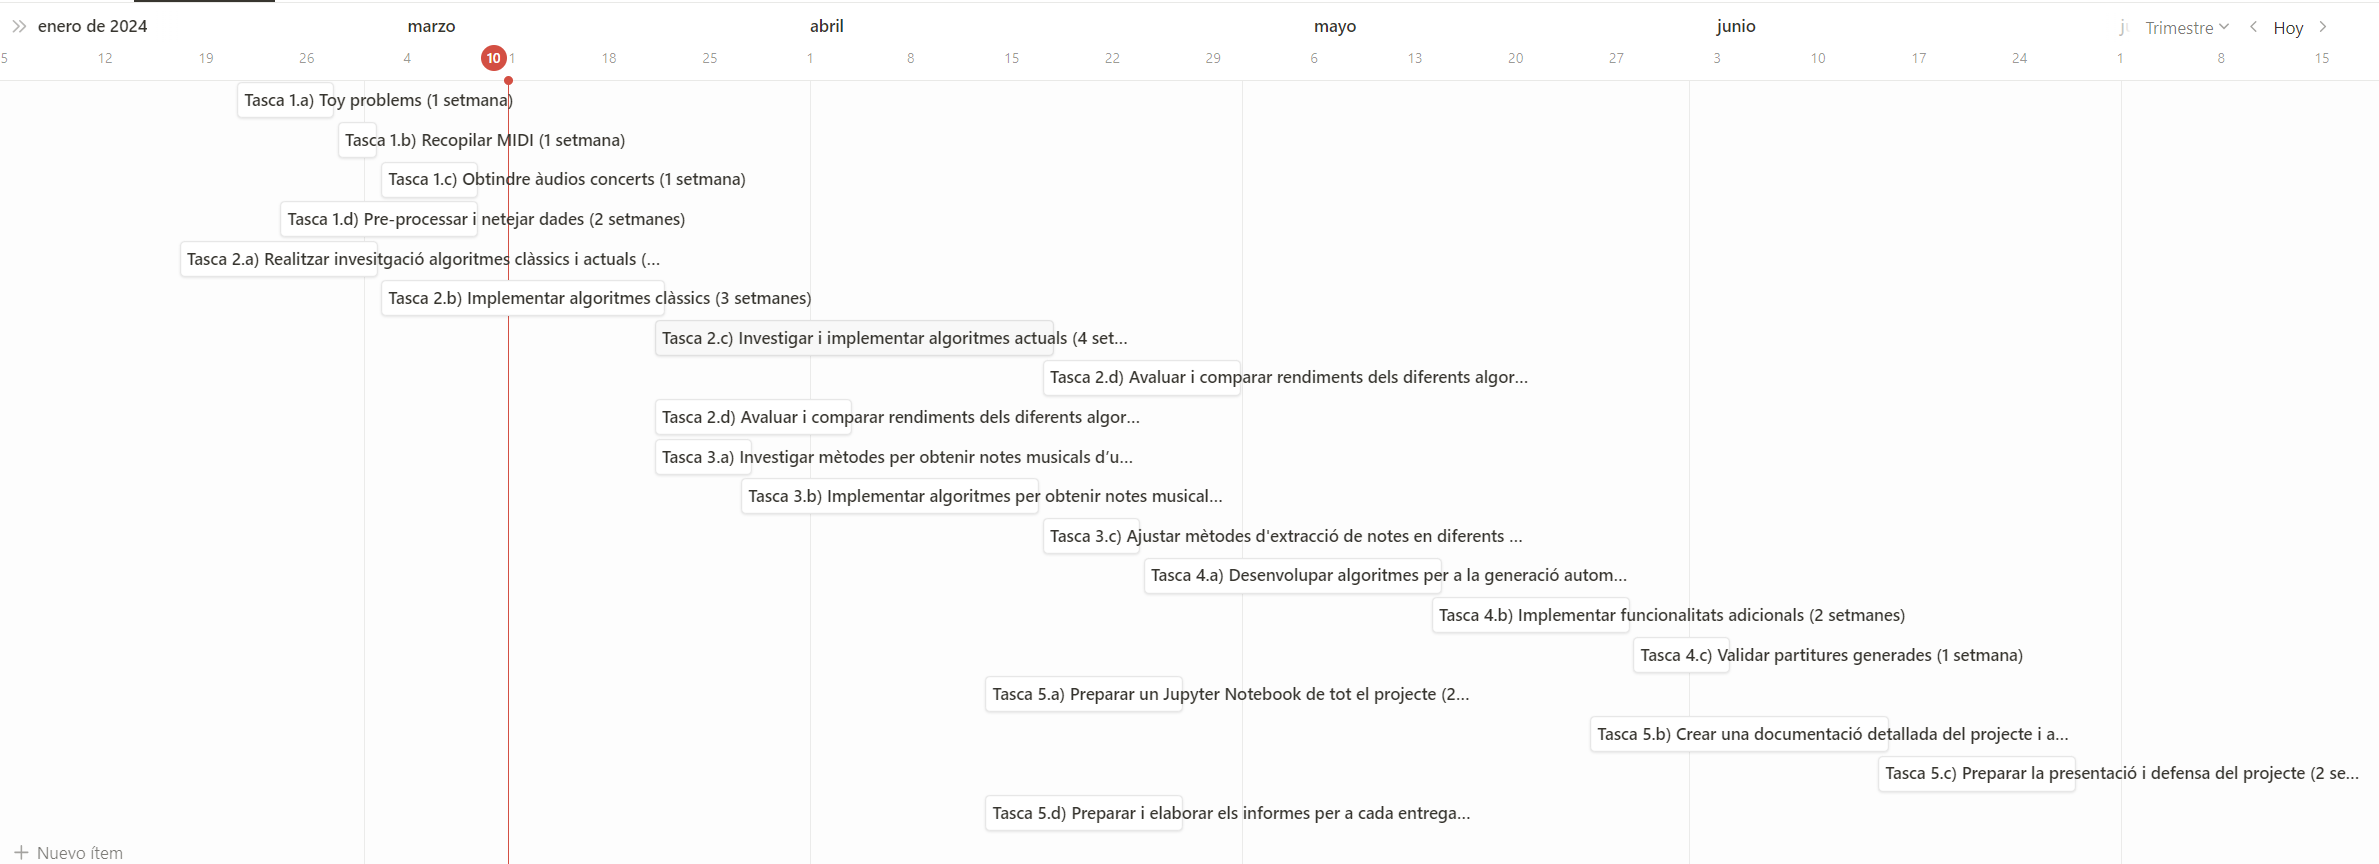
\includegraphics[width=\textwidth]{img/Diagrama de Gantt Claro Fecha.png}
    \caption{Diagrama de Gantt del projecte.}
    \label{fig:gantt}
\end{figure*}

Com es pot observar, les tasques de l'apartat 5 (documentació) són més paral·leles, és a dir, realment s'aniran realitzant durant el desenvolupament del projecte.
En total s'ha aconseguit ajustar en el plaç de temps donat tot i que per a aconseguir-ho s'haurà de realitzar alguna hora extra, sobretot en la part inicial del projecte.

\section{Desenvolupament}

El desenvolupament del projecte s'ha separat en 4 grans apartats. Inicialment, la generació i neteja de dades, a continuació, la separació d'àudio en pistes, continuant amb l'anàlisi de la pista obtenint les notes en format MIDI per a finalment generar la partitura donat aquest arxiu.

\subsection{Dades}
Les dades es separen en diferents grups segons la finalitat d'utilització de les mateixes.

\subsubsection{Elements Simples i Toy Problems}

Els elements simples consisteixen en sons senzills d'un mateix instrument tocant una sola nota o una melodia simple. La duració màxima d'aquestes dades és de 5 segons.

Aquests elements simples s'introdueixen en un bloc de codi que anomenem "generador". Aquest generador agrupa un o més elements simples per generar els \textbf{Toy Problems}. Els Toy Problems són el resultat d'agrupar els elements simples i modificar-los mitjançant els valors de diverses variables del generador. Les variables d'ajust són: \(\alpha\), \(\beta\), volum1 i volum2, amb les quals es crea i modifica un àudio estèreo per variar el volum dels canals dret i esquerre. Aquests valors permeten generar moltes dades diferents amb pocs recursos (elements simples). Per mantenir la base de dades senzilla i de petites dimensions, els Toy Problems no s'enregistren; simplement s'enregistra la seva llavor (seed) de creació, que consta dels valors de les variables i dels elements simples utilitzats.

L'esquema de creació del Toy Problem és el següent: \ref{fig:data-generator-formula}
\begin{figure}[h]
    \centering
    
\includegraphics[width=1\linewidth]{img/data_generator_formula.png}
    \caption{Esquema de creació de Toy Problems}
    \label{fig:data-generator-formula}
\end{figure}

\subsubsection{Elements Complexos i Problemes Complexos}

Els elements complexos, de manera similar als Toy Problems, es generen per formar els \textbf{problemes complexes}. Aquests problemes estan formats per melodies més complexes amb l'objectiu de tenir àudios d'entrenament més fidels a la realitat, com ara cançons del mercat o similars.

\subsubsection{Àudios Reals}

Els àudios reals consisteixen en enregistraments d'àudios com concerts, gravacions de mòbil, etc. Aquest tipus de dades només s'utilitzen per a la part de test, ja que el model no s'entrena amb aquestes dades.

En resum, el projecte utilitza 5 tipus de dades, dels quals 3 s'utilitzen per entrenar, validar i testar el model, i 1 només per a la part de test. Els 2 tipus de dades restants són elements utilitzats per generar les dades d'entrenament, validació i test.



\subsection{Separació d'àudio}

Per a la separació d'àudio, s'aplicaran dos mètodes diferents amb l'objectiu d'analitzar i comparar els resultats obtinguts.

El primer mètode utilitzat serà el mètode clàssic, basat en l'algoritme de Independent Component Analysis (ICA). L'ICA és un mètode amplament utilitzat per a la descomposició de l'audio en les seves fonts originals. Aquest algoritme té com a objectiu la separació de les senyals d'entrada en diferents components independents. En aquest cas, s'utilitzarà l'ICA per aconseguir la separació d'un àudio en pistes individuals.

D'altra banda, s'aplicarà un segon mètode basat en tècniques de Machine Learning (ML). En aquest cas, es farà servir una arquitectura de xarxa neuronal convolucional (CNN) coneguda com a U-Net \cite{spleeter2020}. La U-Net és àmpliament utilitzada en tasques de processament d'àudio i imatge per a la segmentació i reconstrucció d'imatges. Tot i que la U-Net és l'opció principal, es considerarà l'ús d'altres arquitectures de xarxes neuronals si es considera més convenient per al projecte.

Per a poder analitzar el rendiment d'aquests mètodes amb les màximes variacions possibles, s'utilitzaran diverses formes de processament d'àudio, que es programaran com a "caixes" o funcions per a permetre el seu fàcil intercanvi per tal de poder comparar els resultats finals i analitzar en quins casos funciona millor una forma de processament o si una d'elles destaca notablement respecte les altres. 

Aquestes formes de processament inclouran \cite{audio-processing-ML}:

\begin{itemize}
\item \textbf{Spectrum:} Anàlisi de l'espectre de freqüències de l'àudio.
\item \textbf{Cepstrum:} Anàlisi del cepstre de l'àudio, utilitzat per a la representació de la informació d'una manera més robusta enfront de la reverberació i el soroll.
\item \textbf{MFCC (Mel Frequency Cepstral Coefficients):} Coeficients cepstrals de les freqüències mel, amplament utilitzats en el reconeixement de veu i altres tasques de processament d'àudio.
\item \textbf{GFCC (Gammatone Frequency Cepstral Coefficients):} Coeficients cepstrals de les freqüències gammatone, una representació més semblant al processament auditiu humà.
\end{itemize}

Aquestes formes de processament permetran una anàlisi detallada dels resultats obtinguts mitjançant diferents mètodes i tècniques, ajudant a determinar quin és l'approach més adequat per al problema de separació d'àudio en el marc d'aquest projecte.

\subsection{Anàlisi de resultats (Temporal)}

De moment no està pensat del tot aquest apartat, per tant la informació d'aquest és temporal i susceptible a canvis.

La idea principal és obtenir els resultats del punt anterior i guardar-los de manera automatitzada guardant la seed de generació de les dades d'entrada, el processament de dades i algorisme utilitzat i alguns hiperparàmetres importants per tal de poder replicar els resultats en un futur en cas de voler estudiar més un cas.

Una vegada obtingut això, per a cada experiment (Toy problems, problemes complexes i àudios reals), es calcularan algunes mètriques (les quals estàn per decidir encara) per tal de realitzar una avaluació no supervisada.

Addicionalment també es realitzarà una avaluació supervisada per mi mateix on assignaré un valor segons el rang correctesa de la separació d'àudio.

\subsection{Transcripció d'àudio}

Donada una de les pistes obtingudes en la separació d'àudio, és a dir un sol instrument, es realitza una transcripció de les notes en format MIDI. D'aquesta manera, es coneix la durada de cada nota i la seva posició temporal. \cite{music-transcription-app132111882} 

Per al desenvolupament d'aquesta part m'he basat en Omnizard \cite{Omnizard-Wu2021}, doncs ha estat amb el que he obtingut millors resultats.


\subsection{Generació de partitura}

Per a la generació de partitures, he estat fent recerca i provant les llibreries music21 \cite{music21-conf/ismir/CuthbertA10} i partitura \cite{partitura_mec}.

En aquest context, s'ha obtingut millors resultats amb la llibreria music21, però s'explorarà amb més profunditat la llibreria partitura.

L'objectiu d'aquesta subsecció és generar la partitura de cada pista o instrument obtingut mitjançant el procés de separació d'àudio.


\section{Resultats}

Actualement, s'ha aconseguit realitzar l'esquelet de tot el procés, és a dir, donat un àudio, s'obtenen diverses pistes amb els diversos instruments. Una vegada obtinguts, si s'introdueix un àudio, mitjançant Omnizard (que permet introduir links de Youtube o arxius .mp3), s'obté la pista en format MIDI. Finalment, amb la llibreria Music21, s'obté la partitura.

A continuació mostraré links de diversos Google Colab amb exemples d'aquestes proves i resultats, així com algunes imatges.

\subsection{Audio Decomposition Part}

Google Colab: \href{https://colab.research.google.com/drive/1hnlwqaULE_wZDV8ZtSGldOrITDW8WQJs?usp=sharing}{Google Colab Audio Decomposition Part}
En aquesta part, s'introdueix un àudio, que per a l'exemple és de 10 segons, i mitjançant Spleeter \cite{spleeter2020}, es separa en les diverses pistes.

També es pot veure que vaig intentar realitzar una integració amb Omnizard però va fallar per alguna incompatibilitat. És per això que ho vaig separar amb la següent part.

\subsection{Transcripció musical i generació de partitura}

Google Colab 1: \href{https://colab.research.google.com/drive/1W1kDEtN0w8kRLiUZLePwhXBxqFlJAA4x?usp=sharing}{Transcripció (Generació de fitxer MIDI)}
Google Colab 2: \href{https://colab.research.google.com/drive/1tiGLzMGYfOxaYQx5lRwElC0yLjdWvwAU?usp=sharing}{Generació de Partitura}

Per a seguir amb la segona i última part, mitjançant el Google Colab 1, generem l'arxiu en format MIDI donat un arxiu MP3 o un link de Youtube.
La prova la vaig realitzar amb aquest link: \href{https://www.youtube.com/watch?v=aCUI6dNECeA&ab_channel=tocapartituras.com}{Link cançó piano YT}

Com es pot observar, s'obté un fitxer MIDI de manera correcta. El que vaig fer a continuació va ser obrir i escoltar aquest arxiu i tret d'algunes diferències, en general el resultat era bastant fidedigne amb l'original.

A continuació, mitjançant el Google Colab 2, introduim el fitxer prèviament generat (MIDI) per a obtenir la respectiva partitura.
Imatge de la partitura original: \ref{fig:paritura-original}
\begin{figure}
    \centering
    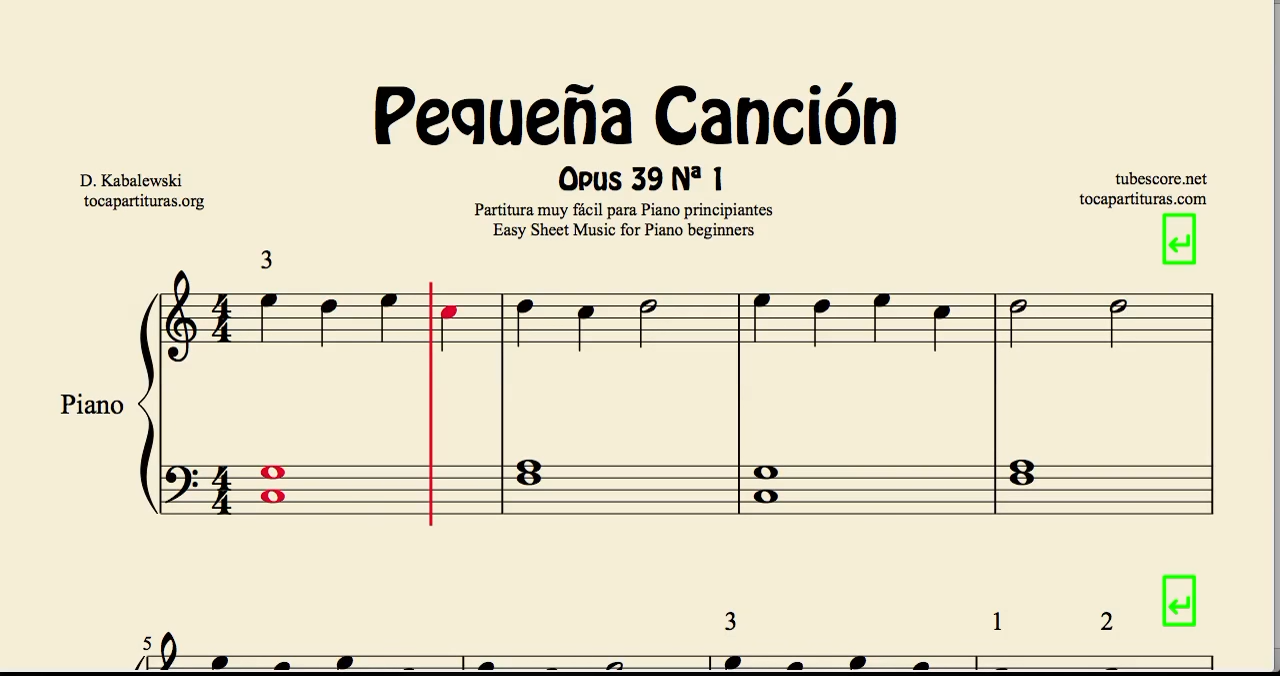
\includegraphics[width=1\linewidth]{img/screenshot-partitura-correcta.png}
    \caption{Partitura original del video de YouTube}
    \label{fig:paritura-original}
\end{figure}

I a continuació podem veure la partitura generada: \ref{fig:partitura-resultat}
\begin{figure}
    \centering
    
\includegraphics[width=1\linewidth]{img/partitura_resultat.png}
    \caption{Partitura resultant, generada al Google Colab 2.}
    \label{fig:partitura-resultat}
\end{figure}

Com es pot observar, el resultat és desastrós i molt diferent. Tot i això es veu que és possible una generació de partitura, tot i que se li haurà de dedicar més temps a entendre com funciona. Ja que, per exemple, es pot veure que la partitura inicial compta amb melodia en la mà dreta i la mà esquerra. En canvi, en la partitura resultant, només ha considerat la de la mà dreta. Aquest podria ser el punt principal d'error fent que es desquadri tant.

Utilitzant la mateixa llibreria i en un entorn controlat, es pot obtenir un resultat correcte, tal i com es pot veure a continuació: \ref{fig:partiture-example}
\begin{figure}
    \centering
    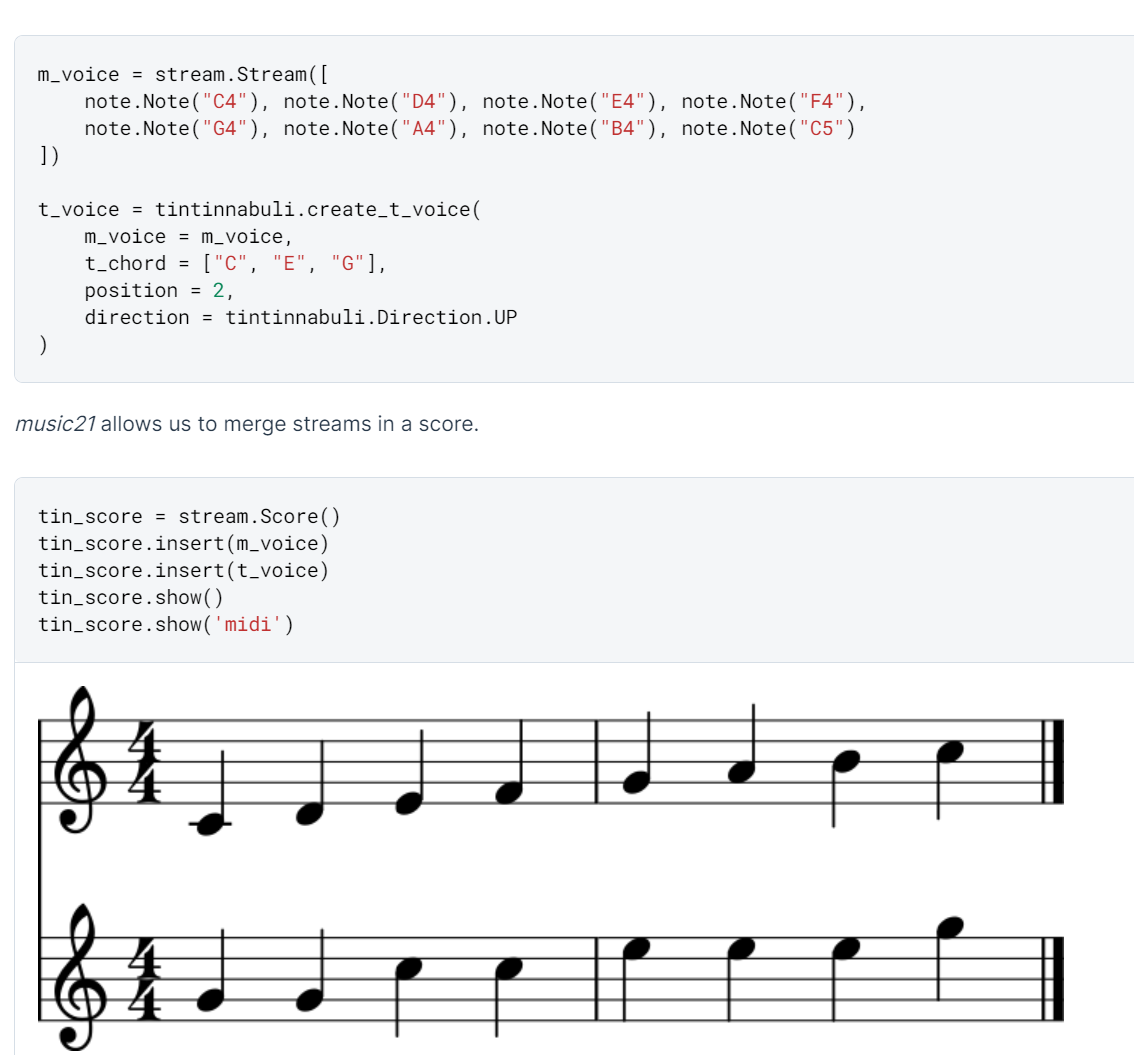
\includegraphics[width=1\linewidth]{img/Partiture-Example.png}
    \caption{Exemple de generació de Partitura en un entorn controlat}
    \label{fig:partiture-example}
\end{figure}

\section{Conclusions}

.... ..  .... .. .... ... ..... ... ..... ... ... ..... .... .
.... ..  .... .. .... ... ..... ... ..... ... ... ..... .... .
.... ..  .... .. .... ... ..... ... ..... ... ... ..... .... .
.... ..  .... .. .... ... ..... ... ..... ... ... ..... .... .
.... ..  .... .. .... ... ..... ... ..... ... ... ..... .... .
.... ..  .... .. .... ... ..... ... ..... ... ... ..... .... .
.... ..  .... .. .... ... ..... ... ..... ... ... ..... .... .
.... ..  .... .. .... ... ..... ... ..... ... ... ..... .... .
.... ..  .... .. .... ... ..... ... ..... ... ... ..... .... .
.... ..  .... .. .... ... ..... ... ..... ... ... ..... .... .
.... ..  .... .. .... ... ..... ... ..... ... ... ..... .... .
.... ..  .... .. .... ... ..... ... ..... ... ... ..... .... .
.... ..  .... .. .... ... ..... ... ..... ... ... ..... .... .
.... ..  .... .. .... ... ..... ... ..... ... ... ..... .... .

\section*{Agraïments}

... ..  .... .. .... ... ..... ... ..... ... ... ..... .... .
.... ..  .... .. .... ... ..... ... ..... ... ... ..... .... .
.... ..  .... .. .... ... ..... ... ..... ... ... ..... .... .
.... ..  .... .. .... ... ..... ... ..... ... ... ..... .... .
.... ..  .... .. .... ... ..... ... ..... ... ... ..... .... .


\bibliographystyle{plain}
\bibliography{biblio}


\appendix

\section*{Apèndix}

\setcounter{section}{1}

\subsection{Secció d'Apèndix}


... ..  .... .. .... ... ..... ... ..... ... ... ..... .... .
.... ..  .... .. .... ... ..... ... ..... ... ... ..... .... .
.... ..  .... .. .... ... ..... ... ..... ... ... ..... .... .
.... ..  .... .. .... ... ..... ... ..... ... ... ..... .... .
.... ..  .... .. .... ... ..... ... ..... ... ... ..... .... .

\subsection{Secció d'Apèndix}


... ..  .... .. .... ... ..... ... ..... ... ... ..... .... .
.... ..  .... .. .... ... ..... ... ..... ... ... ..... .... .
.... ..  .... .. .... ... ..... ... ..... ... ... ..... .... .
.... ..  .... .. .... ... ..... ... ..... ... ... ..... .... .
.... ..  .... .. .... ... ..... ... ..... ... ... ..... .... .


\end{document}

